%!TEX root=./optim_report.tex
\section{Experiments}
\subsection{Deep Learning}
In all our experiments with deep learning models, we saw that for Runge-Kutta methods the training loss decereases extremely fast, as you can see it decreases to near zero in less than $2$ epochs, this phenomenon was observed across all the models we tried but we can not show why we observe and under what conditions are we going to observe.
\\
\\
Another interesting observation we say across all the models we deployed is that the training loss is not too sensitive to changes in the learning rate, in other words for most learning rates the train loss goes to zero and extremely fast.
\\
\\
We also note that RK2 is less noisy compared to Stochastic Gradient Descent, that is the fluctuations in the loss for RK2 have less variance than the fluctuations for the loss in Stochastic Gradient Descent.
\\
\\
However the bad news so far is that despite training loss decreasing extremely fast, it tends to overfit. Here, we observe that if we decay the learning rate fast enough then there is a substantial increase in test performance.
\\
\\
\textbf{ResNet18 on Cifar10} -
Here we compare our optimization scheme with Stochastic Gradient Descent with momentum and learning rate decay.
\\
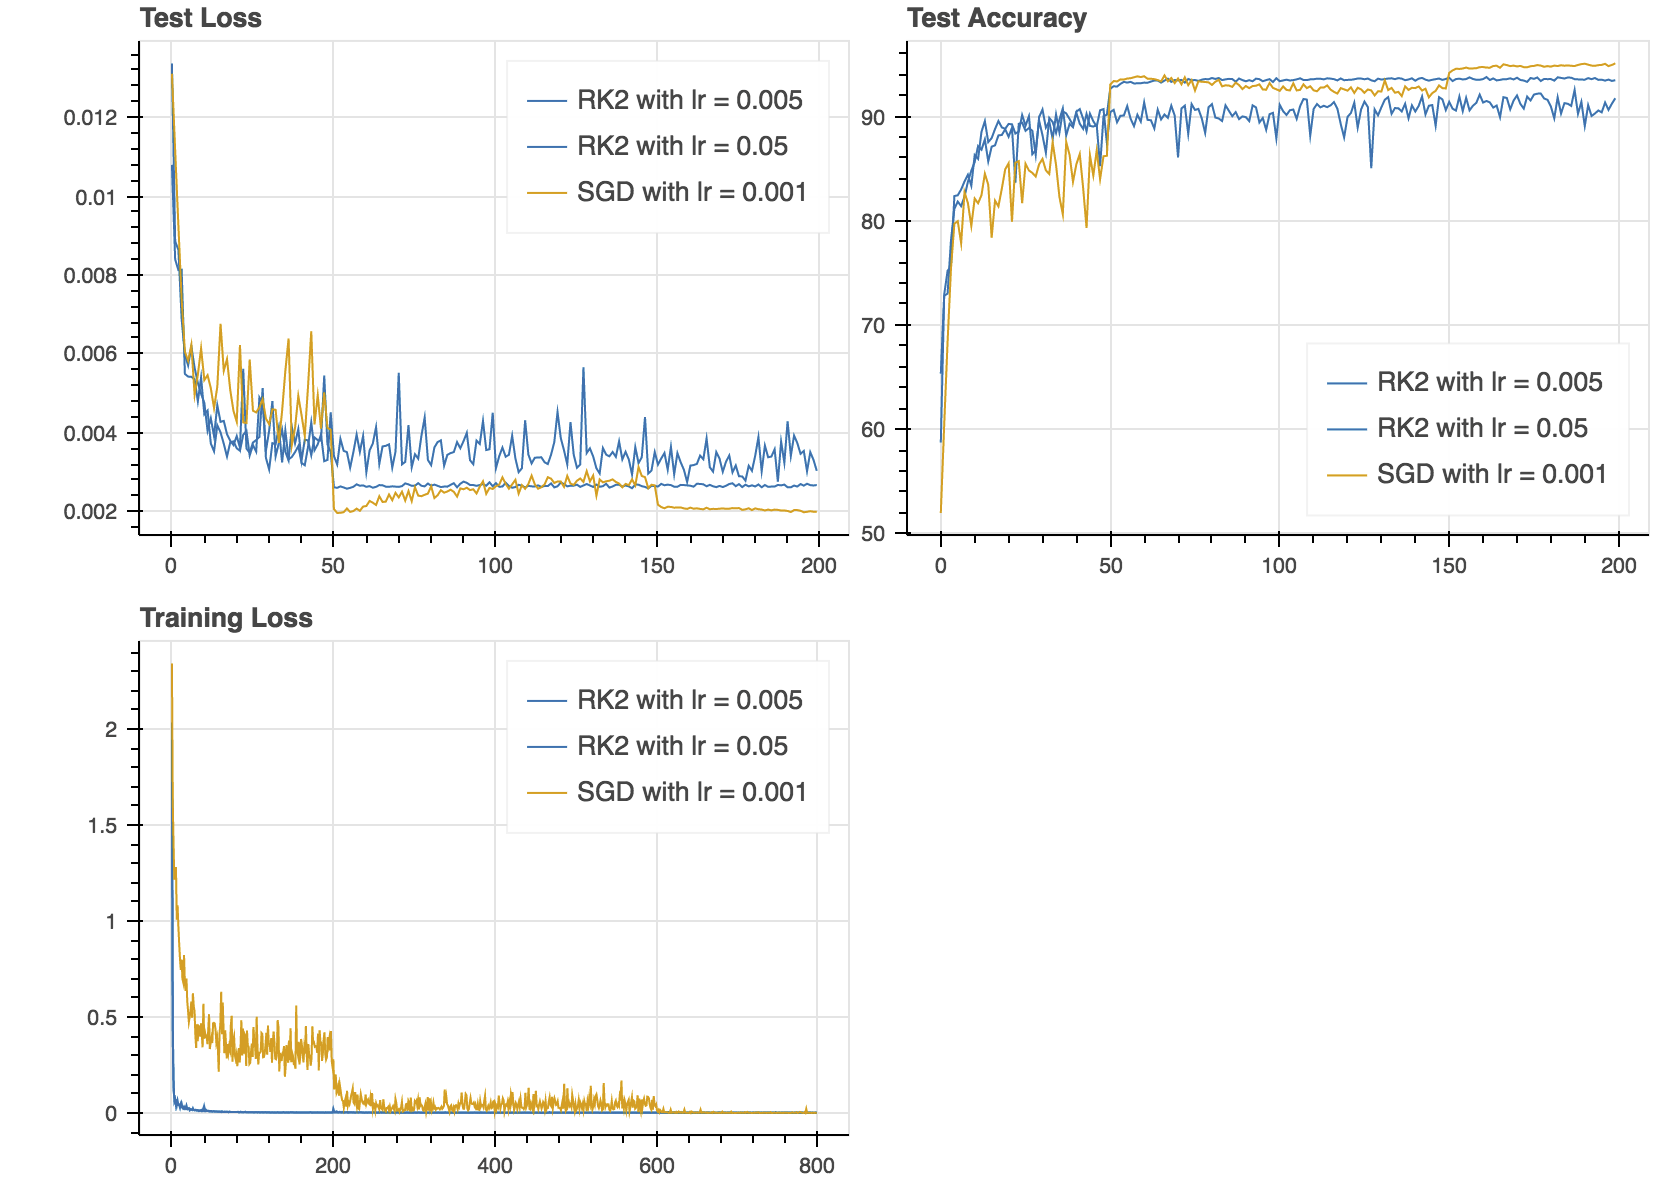
\includegraphics[scale=0.4]{cifar.png}
\\
Now, we compare RK2-Ralston with plain SGD and SGD with momentum
\\
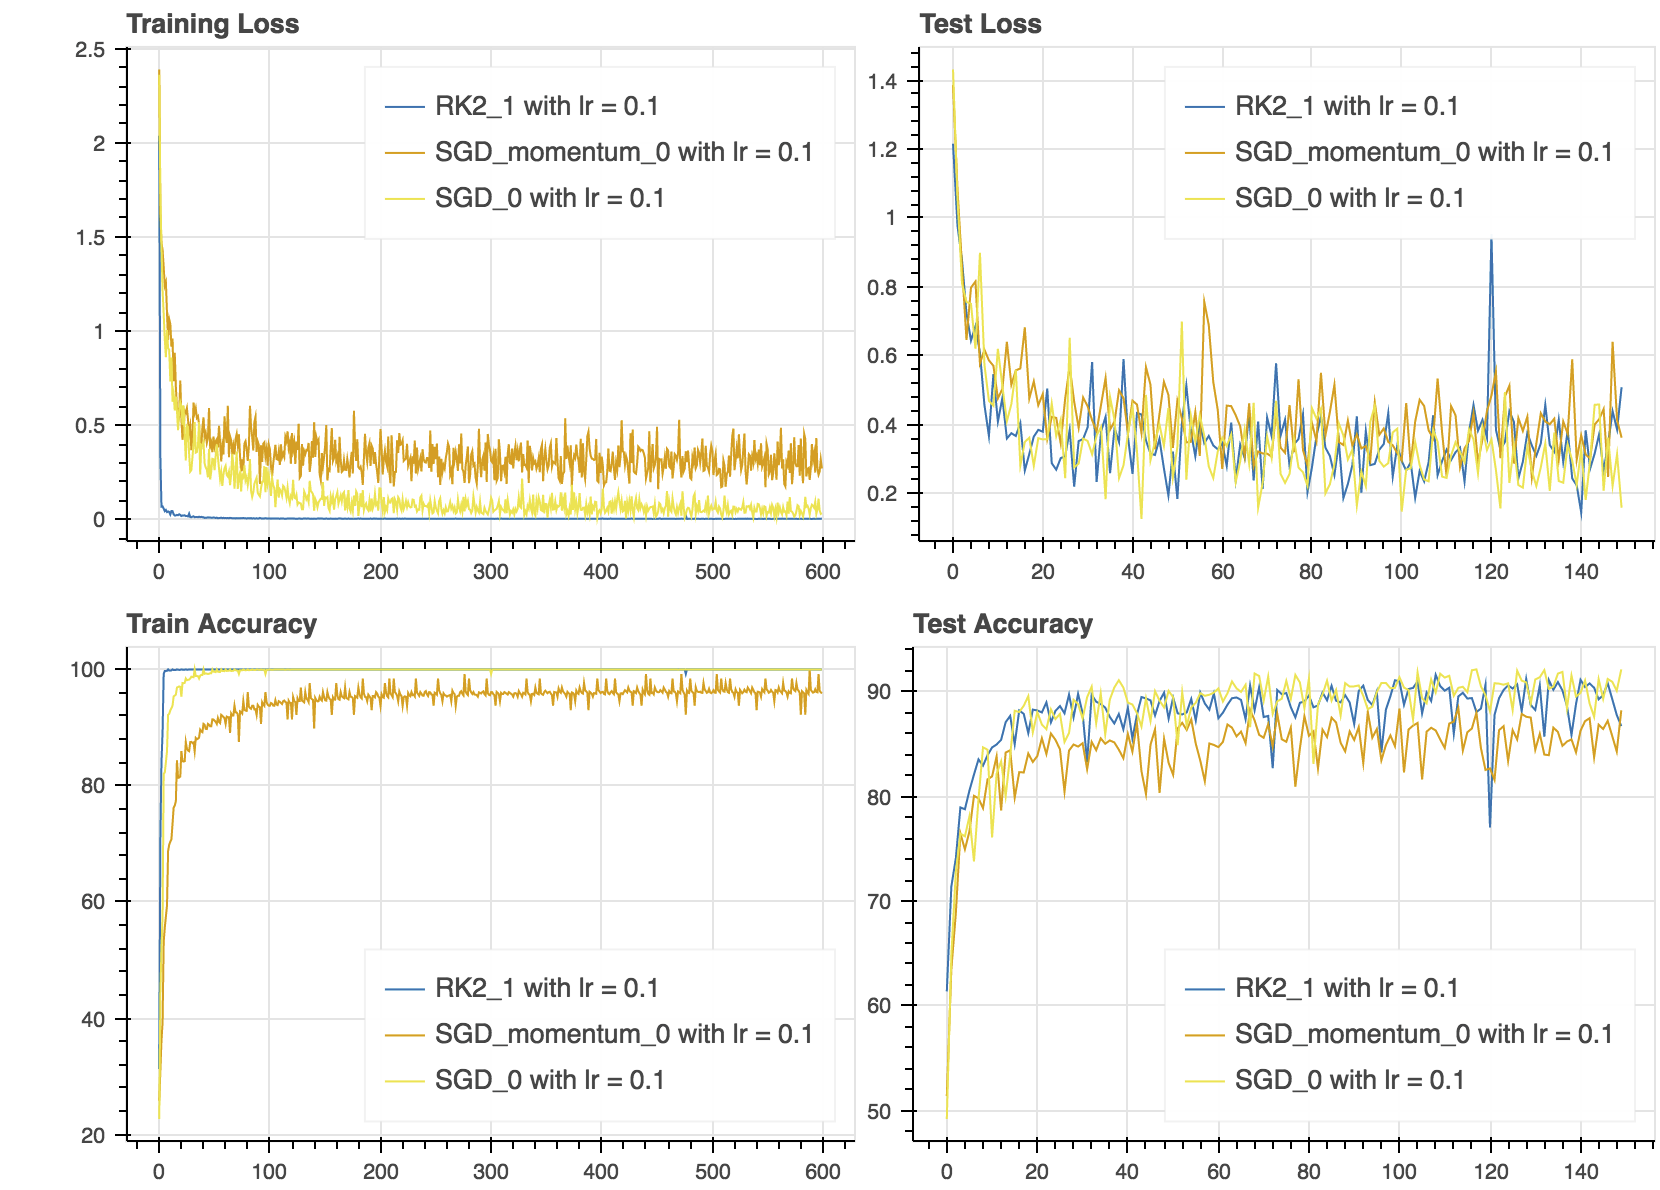
\includegraphics[scale=0.4]{plots/resnet_1.png}
\\
Now, we compare RK2-Heun with plain SGD and SGD with momentum
\\
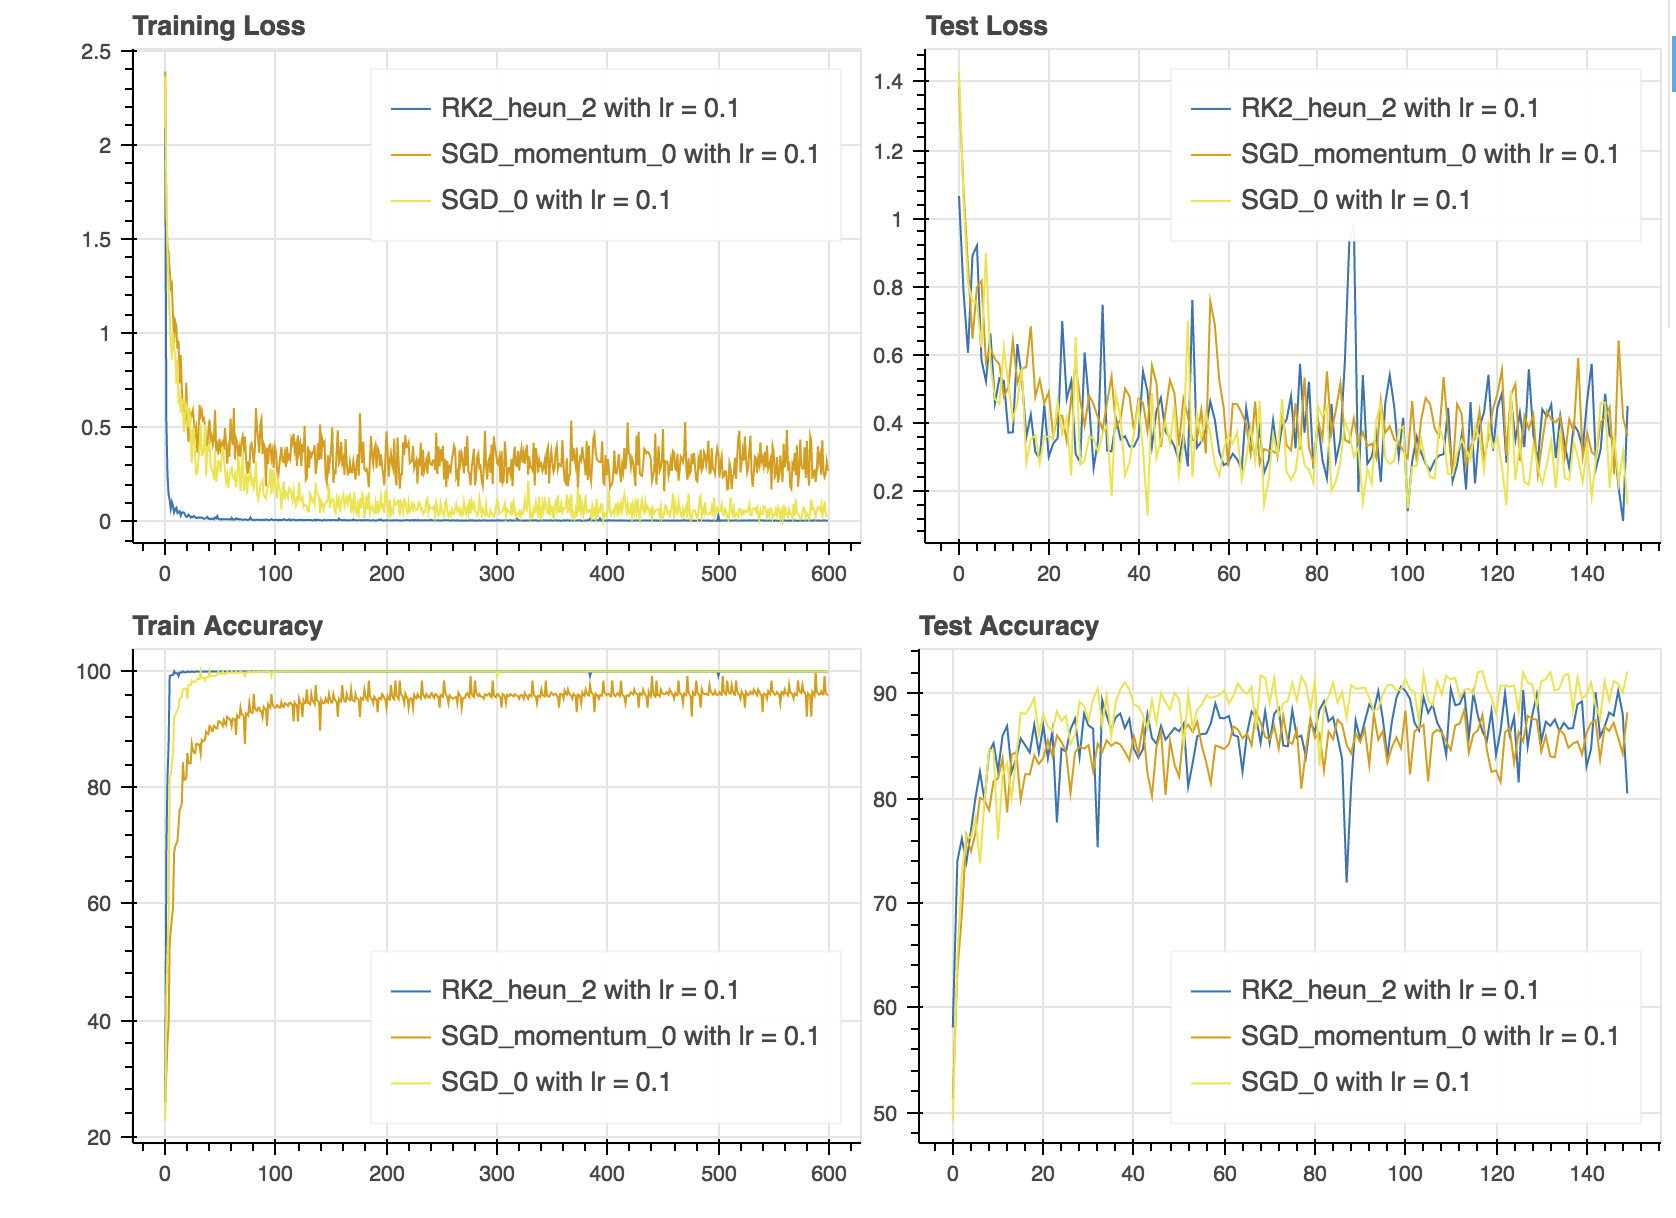
\includegraphics[scale=0.4]{plots/resnet_2.png}
\\
\textbf{WideResnet on Cifar10} -
Here we compare our optimization scheme, Runge-Kutta Ralston Method with Stochastic Gradient Descent. The different Runge-Kutta plots correspond to different learning rate decay schedules and different learning rates. Here again we can say that the variance on the test loss and test accuracy is much less compared to SGD with momentum. And also RK2 is not too sensitive to learning rate changes.
\\
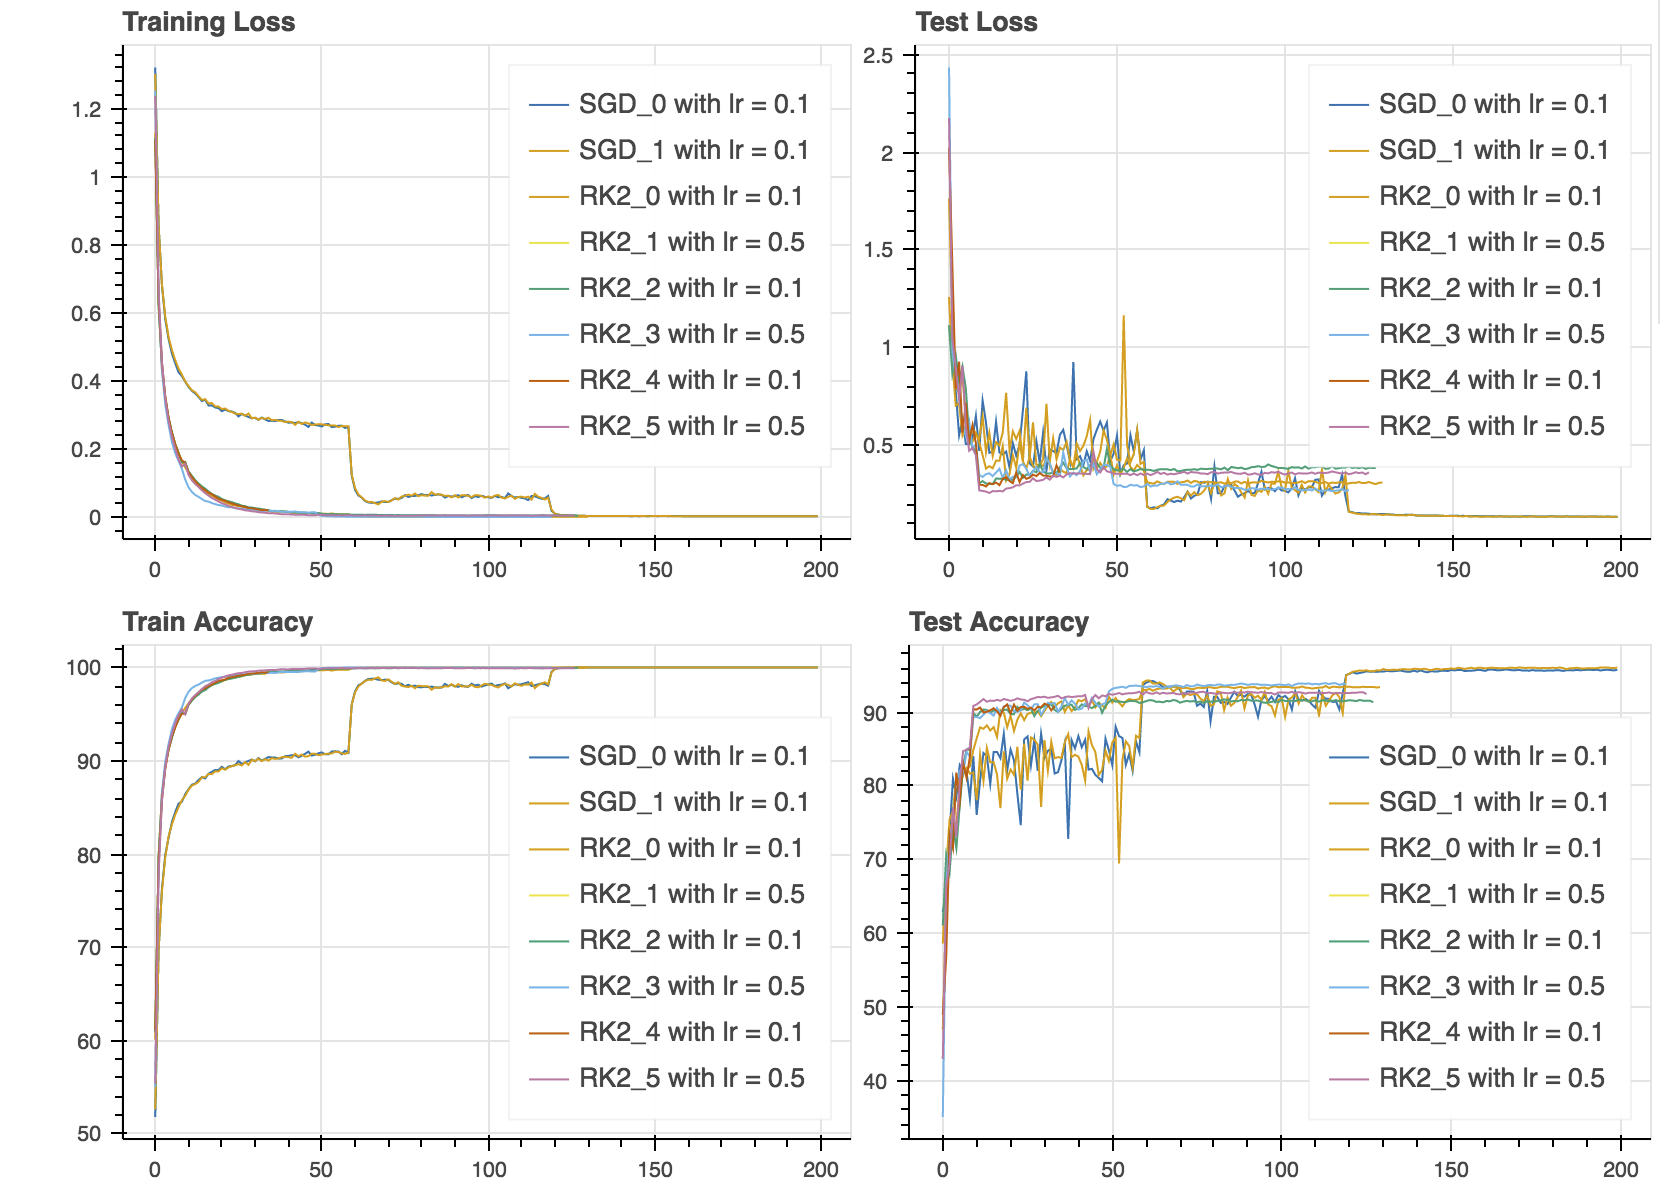
\includegraphics[scale=0.4]{plots/wideresnet.png}

\subsection{Convex Models}

Here we do plain logistic regression and logistic regression with weight-decay on the mnist dataset. A big difference between the the previous experiments and these experiments is that the number of parameters in the model here are less than the number of training samples. So the chances of overfitting are much less. Here we present some plots for the experiments we did with these models.

\subsection{Lasso}
Here we show that our algorithm is not too sensitive to changes in the learning rate
\\
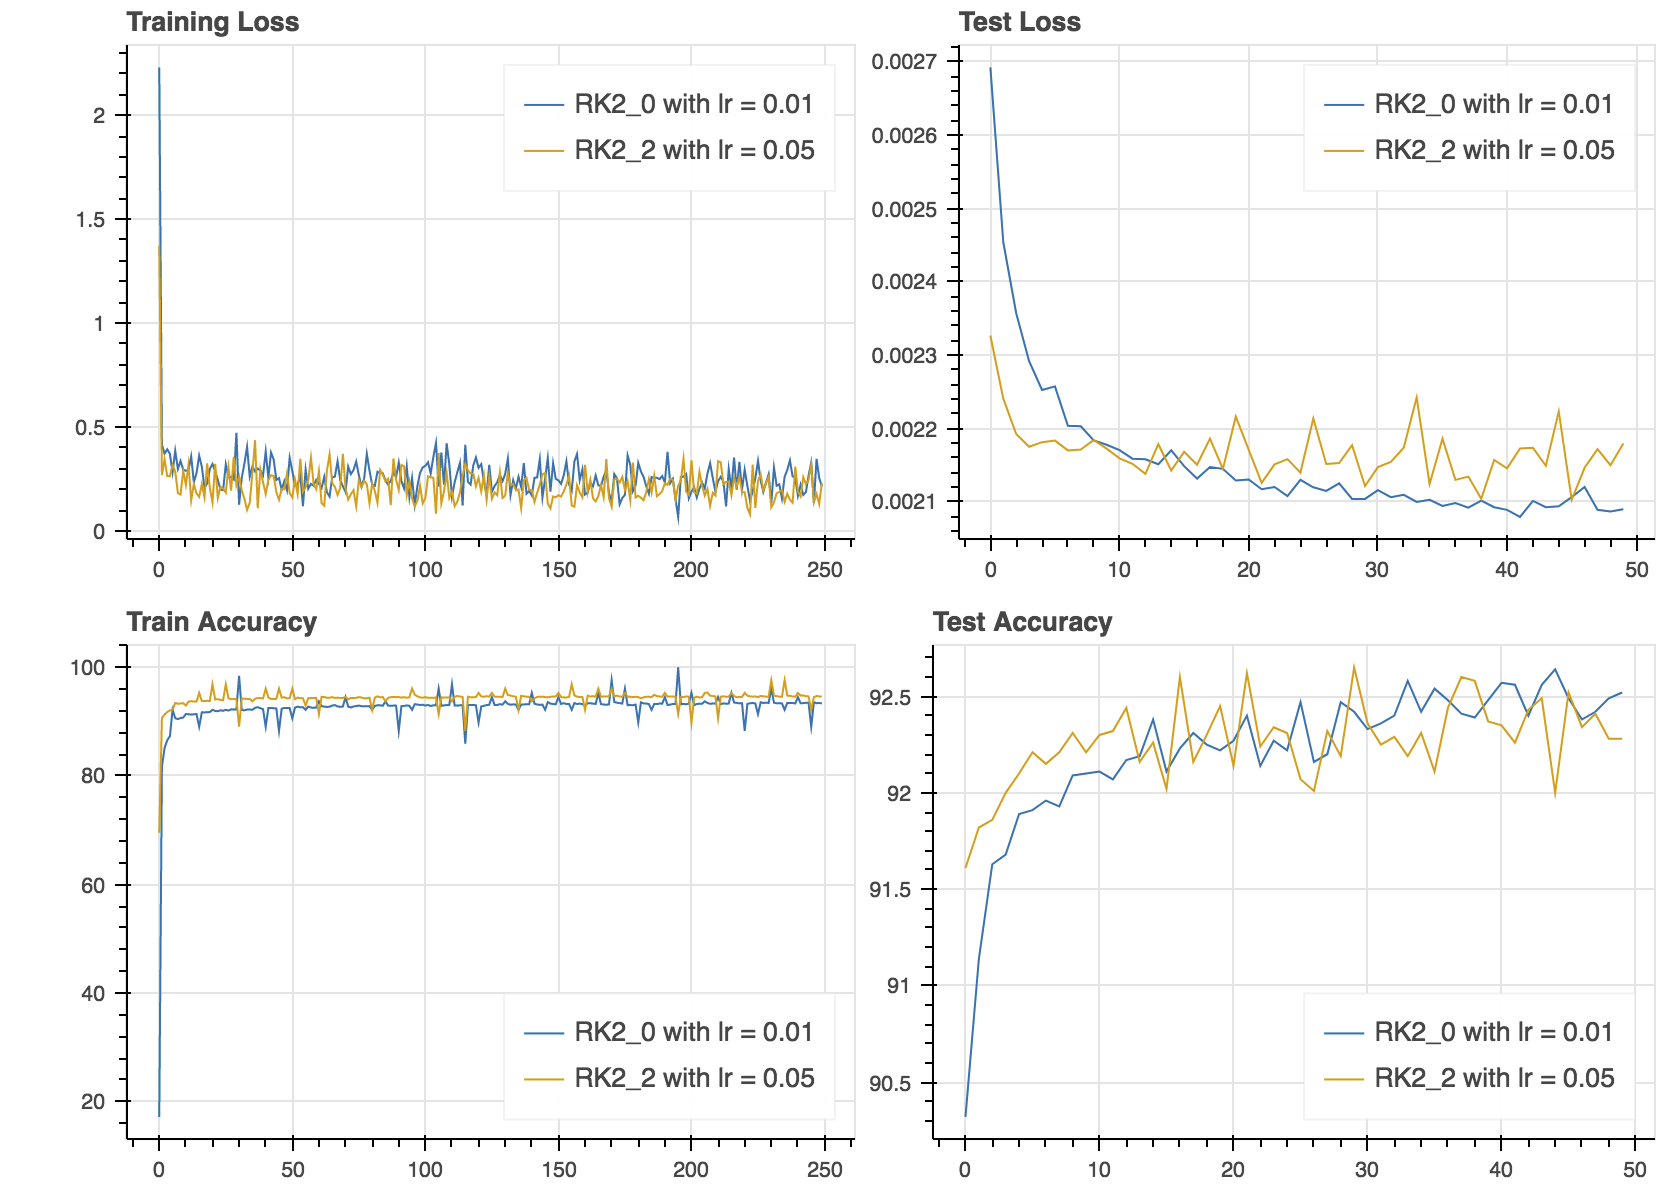
\includegraphics[scale=0.4]{plots/lasso_4.png}
\\
Now, we show plots to compare our optimizer with simple stochastic gradient descent, its variants and Adagrad.
\\
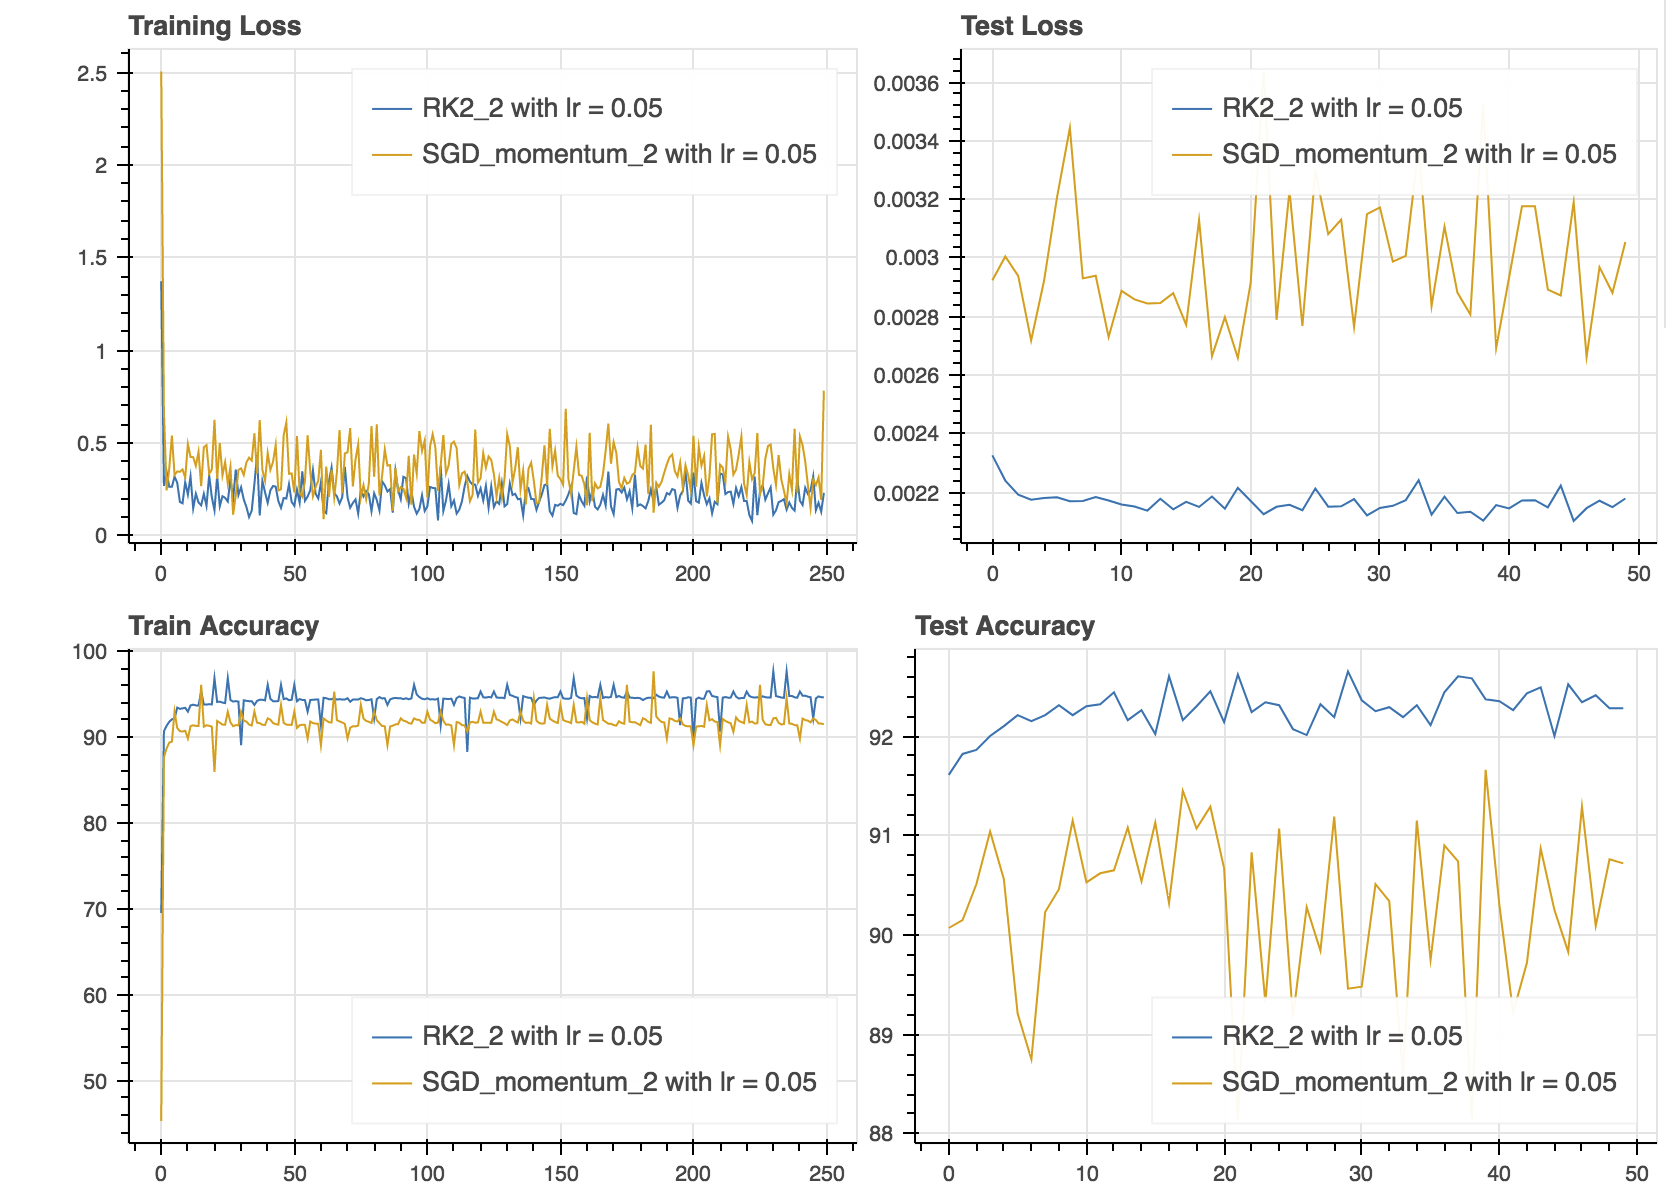
\includegraphics[scale=0.4]{plots/lasso_3.png}
\\
Below we show plots to compare our optimizer with Accelerated stochastic gradient descent.
\\
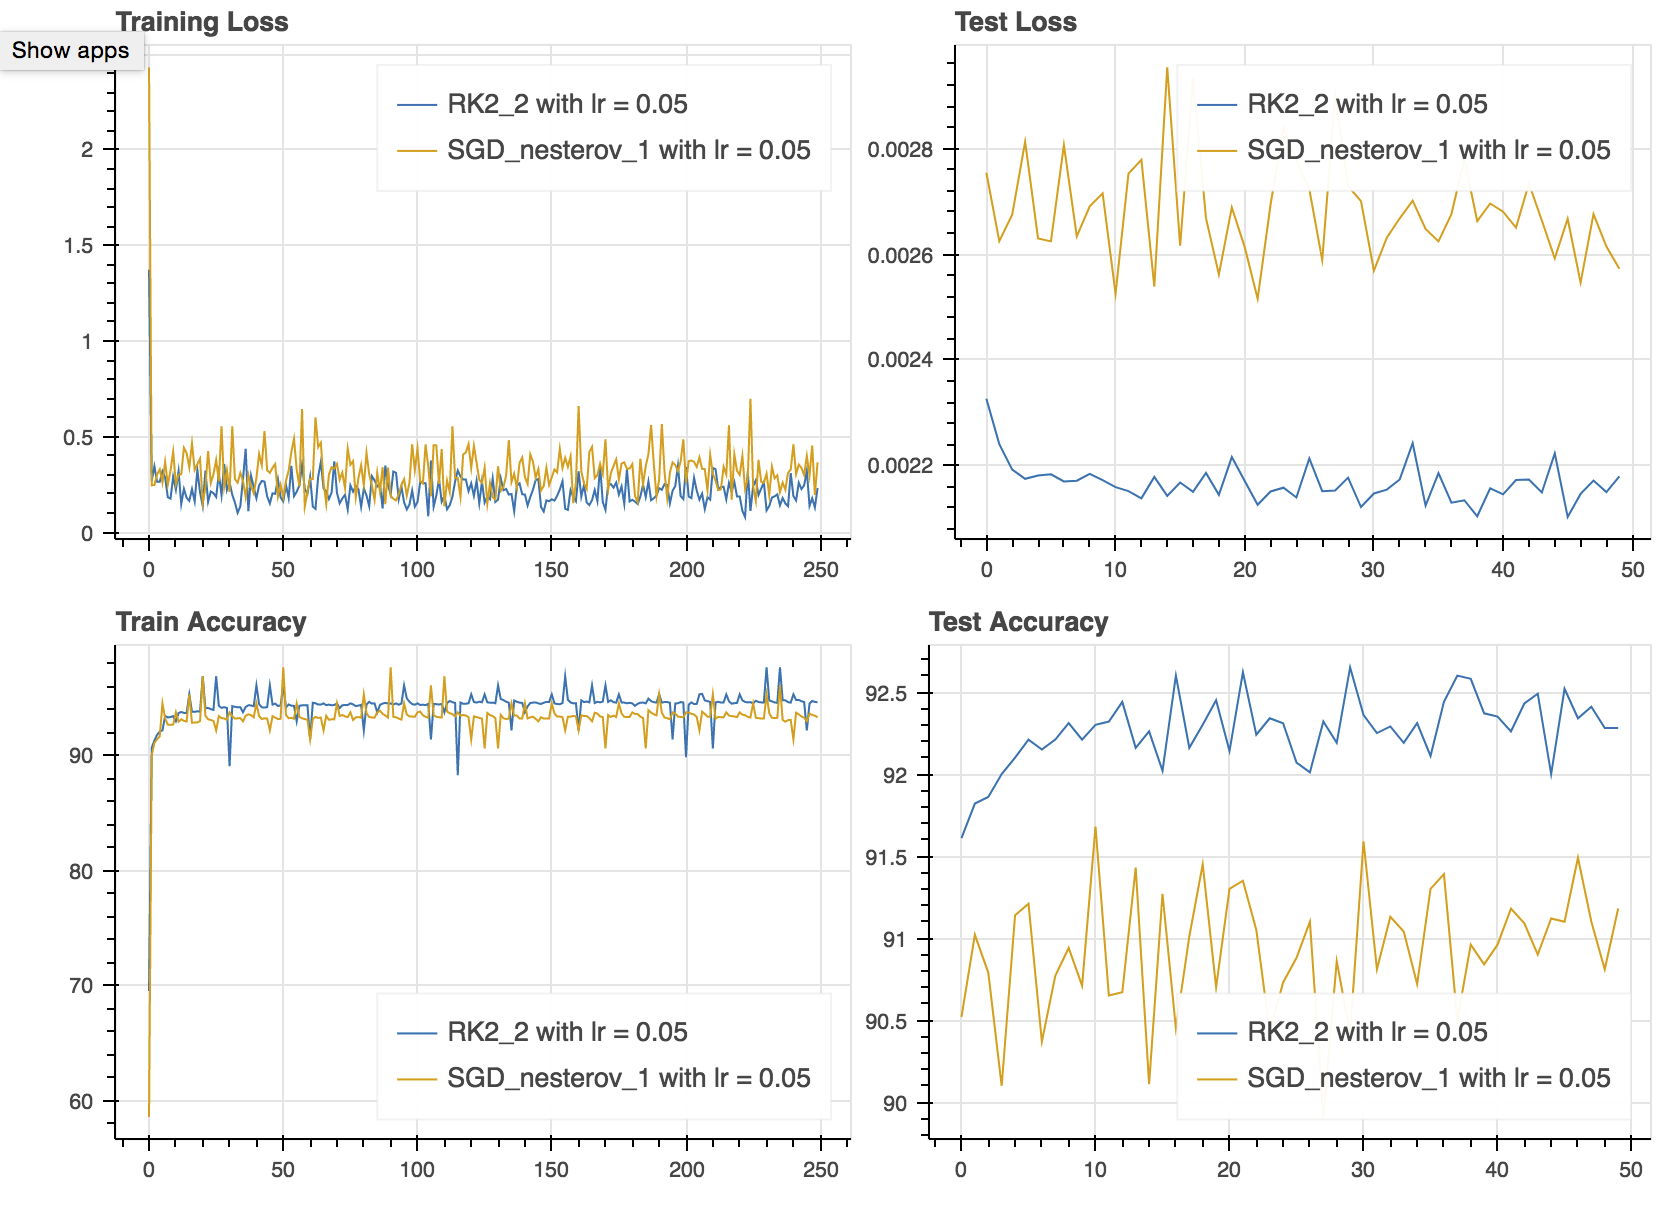
\includegraphics[scale=0.4]{plots/lasso_2.png}
\\
Here we compare a 4th order optimizer based on Runge-Kutta Methods that we wrote with RK2 and SGD
\\
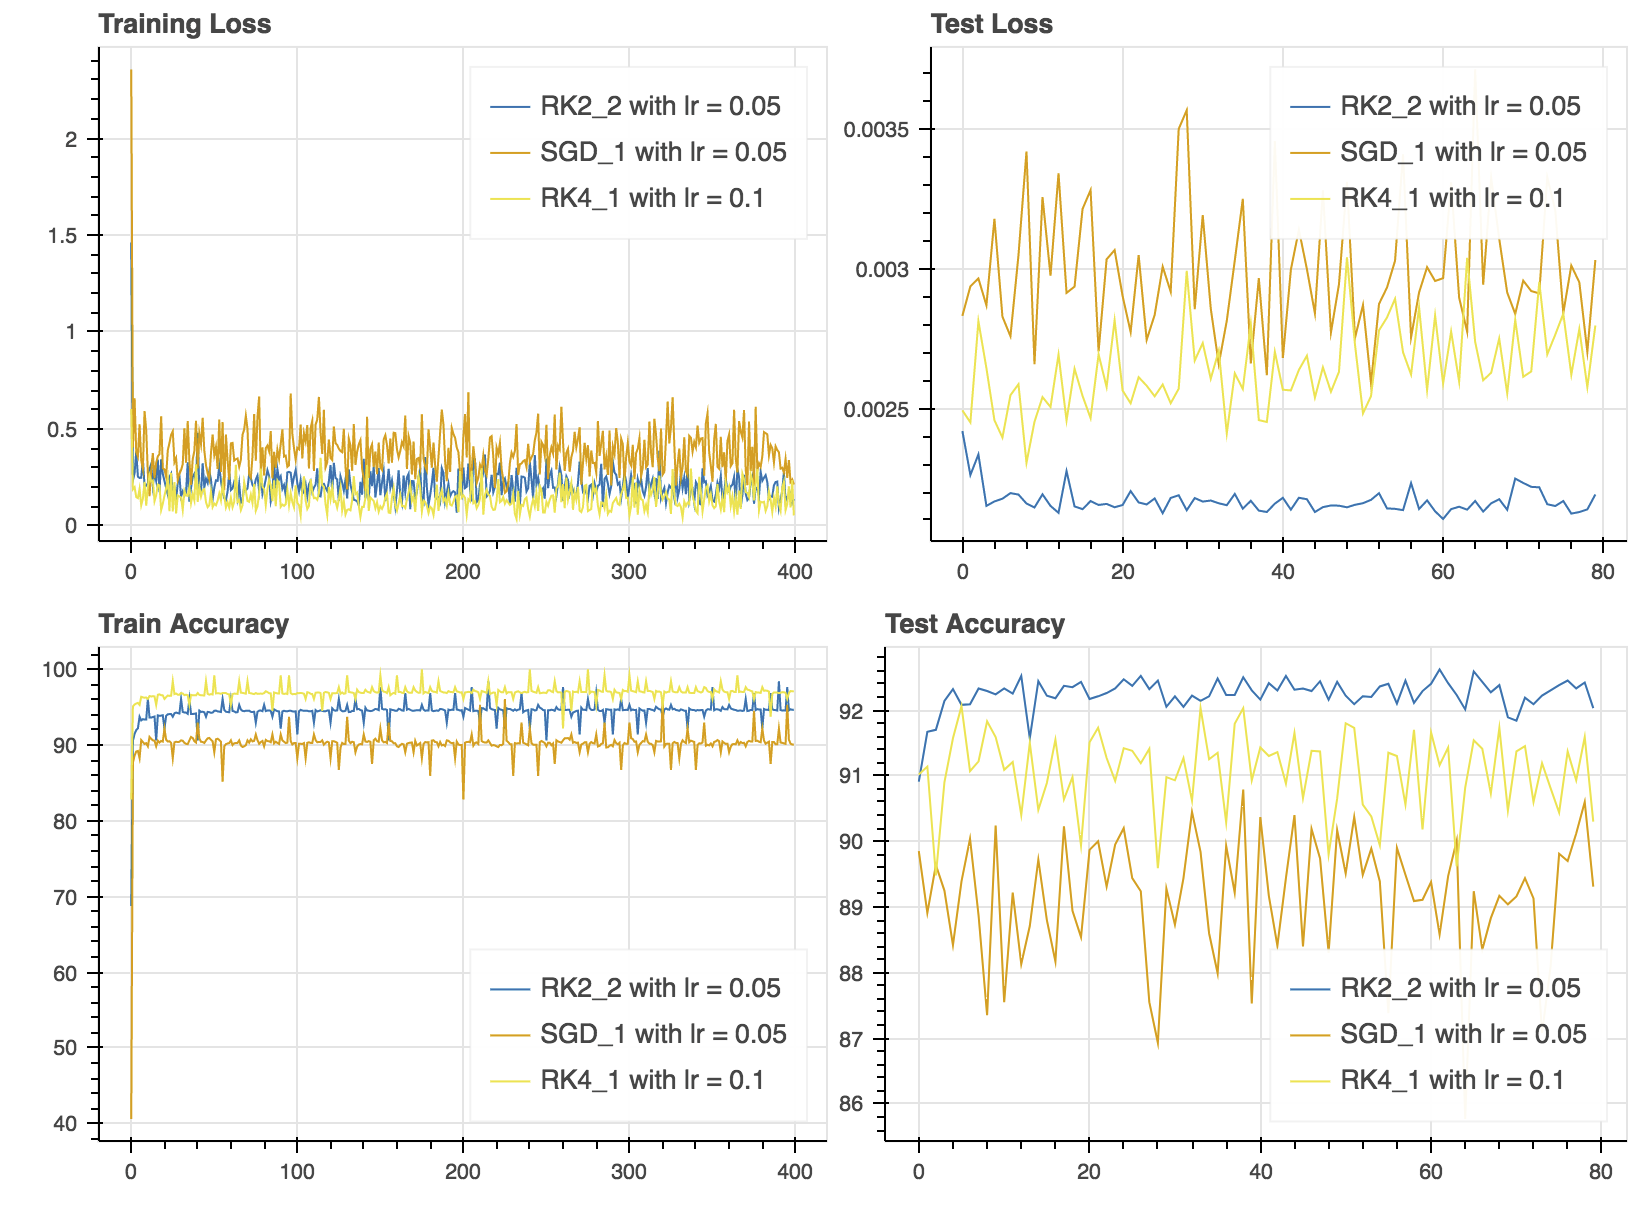
\includegraphics[scale=0.4]{plots/lasso_1.png}
\\

